\chapter{\IfLanguageName{dutch}{Stand van zaken}{State of the art}}
\label{ch:stand-van-zaken}
\graphicspath{{../../Images/}} 
% Tip: Begin elk hoofdstuk met een paragraaf inleiding die beschrijft hoe
% dit hoofdstuk past binnen het geheel van de bachelorproef. Geef in het
% bijzonder aan wat de link is met het vorige en volgende hoofdstuk.

% Pas na deze inleidende paragraaf komt de eerste sectiehoofding.

Dit hoofdstuk bevat je literatuurstudie. De inhoud gaat verder op de inleiding, maar zal het onderwerp van de bachelorproef *diepgaand* uitspitten. De bedoeling is dat de lezer na lezing van dit hoofdstuk helemaal op de hoogte is van de huidige stand van zaken (state-of-the-art) in het onderzoeksdomein. Iemand die niet vertrouwd is met het onderwerp, weet nu voldoende om de rest van het verhaal te kunnen volgen, zonder dat die er nog andere informatie moet over opzoeken \autocite{Pollefliet2011}.

Je verwijst bij elke bewering die je doet, vakterm die je introduceert, enz. naar je bronnen. In \LaTeX{} kan dat met het commando \texttt{$\backslash${textcite\{\}}} of \texttt{$\backslash${autocite\{\}}}. Als argument van het commando geef je de ``sleutel'' van een ``record'' in een bibliografische databank in het Bib\LaTeX{}-formaat (een tekstbestand). Als je expliciet naar de auteur verwijst in de zin, gebruik je \texttt{$\backslash${}textcite\{\}}.
Soms wil je de auteur niet expliciet vernoemen, dan gebruik je \texttt{$\backslash${}autocite\{\}}. In de volgende paragraaf een voorbeeld van elk.

\textcite{Knuth1998} schreef een van de standaardwerken over sorteer- en zoekalgoritmen. Experten zijn het erover eens dat cloud computing een interessante opportuniteit vormen, zowel voor gebruikers als voor dienstverleners op vlak van informatietechnologie~\autocite{Creeger2009}.
\newpage
\section{Versiebeheer}
\subsection{Inleiding}
Versiebeheer is een zeer belangrijk gegeven binnen softwareontwikkeling. Zo waren er maar liefst in totaal een 100 miljoen projecten in 2018 op het populaire versiebeheer platform GitHub \autocite{Git2018}. GitHub is echter niet de enige speler op de markt. Er zijn nog tal van andere bedrijven actief binnen versiebeheer.Toch is het interessant om even stil te staan en de vraag te stellen: welke problemen lost versiebeheer effectief op?

Stel volgende scenario: Alice en Bob zijn aangenomen om te werken voor Bedrijf X. Hun eerste taak is een website ontwikkelen voor een T-Shirt Webshop. Ze zetten samen hun project op, bespreken de verschillende technologieën en gaan zelfstandig aan de slag. Op het einde van de dag hebben ze elk een verschillende pagina gemaakt en deze willen ze graag met elkaar delen. Een naïeve oplossing zou om de bestanden met elkaar uit te wisselen via mail of fysieke hardware. Dit kost echter veel tijd en de code die geschreven wordt zit verspreid over twee personen. Mocht Bob de code kwijtraakt door een defect dan zal deze opnieuw moeten geschreven worden. Een betere oplossing zou zijn om het project op een centrale server te gaan opslaan. Bob en Alice passen dan bestanden aan op deze centrale  server en hebben op die manier ook altijd toegang tot elkaars werk.

Door deze manier van werken is er een nieuw probleem. Alice kan een fout opslaan waardoor Bob zijn code niet meer werkt. Als deze fout vervolgens op de centrale server komt te staan werkt de gehele website niet meer. Om dit probleem te voorkomen wordt er gebruik gemaakt van het concept van \textbf{versies}. Elke aanpassing die er centraal gebeurd resulteert in een nieuwe versie van het project. Men kan altijd terugkeren naar een eerdere versie.

\textcite{Loeliger2009} stellen dan ook dat een versiebeheersysteem een middel is om verschillende versie van code te gaan beheren en bijhouden.De auteurs geven dan ook volgende drie eigenschappen waaraan elk systeem beantwoord:

\begin{itemize}
	\item Het bijhouden en ontwikkelen van een centraal archief
	\item Het bijhouden en toegang verschaffen van oudere versies van dit archief
	\item Het noteren van alle veranderingen van het archief in een centraal logboek.
\end{itemize}

Versiebeheer is geen nieuw concept. Er zijn zoals eerder aangehaald verschillende Software suites. Toch zijn er volgens \textcite{Chacon2014} drie grote categorieën die we kunnen onderscheiden:

\begin{itemize}
	\item Lokale versiebeheersystemen. De veranderingen in de bestanden die worden aangebracht worden lokaal op de computer bewaard in bijvoorbeeld een Database. Een gekend voorbeeld hiervan is RCS (Revision Control System). Dit is zeker een eenvoudige oplossing om verschillende versies te gaan bijhouden. Toch leent deze manier van werken zich niet voor bestanden te delen of samen te gaan werken aan een project.\\
	
\begin{figure}[h!]
	\centering
	\caption[Overzicht structuur Lokale VCS]{Overzicht van de structuur van een Lokale VCS.}
	\label{fig:lvcs}
	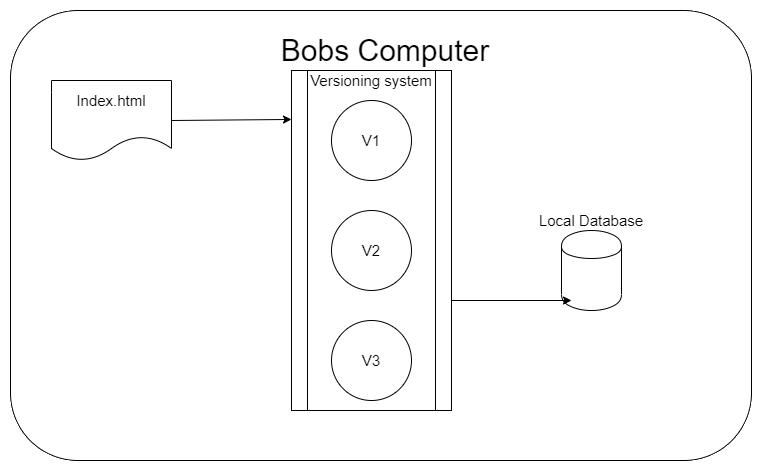
\includegraphics[scale=0.5]{LVCS.png}
\end{figure}

	\item CVCS: Om samen te kunnen werken aan dezelfde bestanden kan er geopteerd worden voor een CVCS (Centralised Version Control System). In plaats van de database lokaal bij te gaan houden maken we gebruik van een centrale server. Wil Bob bijvoorbeeld aan bestand A zal hij lokaal een kopie gaan maken van dit bestand en vervolgens de veranderingen doorsturen naar de centrale database. \\ 

Een ander voordeel van deze manier van werken is dat men de centrale database kan gaan afschermen. Op deze manier krijgen mensen enkel toegang tot de bestanden die men nodig heeft.\\

\begin{figure}[h!]
	\centering
	\caption[Overzicht structuur CVCS]{Overzicht van de structuur van een CVCS.}
	\label{fig:lvcs}
	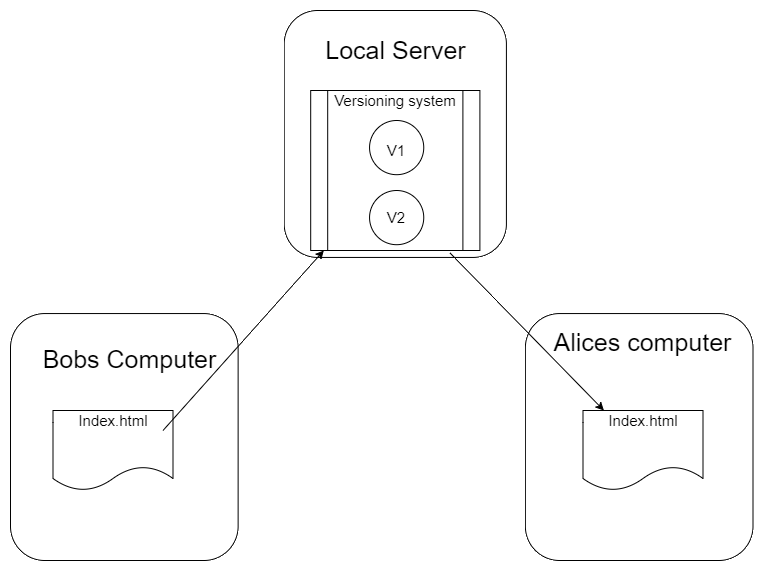
\includegraphics[scale=0.5]{CVCS.png}
\end{figure}

	\item DVCS: Een nadeel van alles centraal te gaan beheren is het zogenaamde \textit{single point of failure(SPOF)} probleem. Een SPOF is een onderdeel van een systeem dat mocht het uitvallen heel het systeem tot een halt roept. Er zijn drie types van SPOF: hardware, software en database. Een mogelijke oplossing voor dit probleem is redundantie, wat wilt zeggen het aanbieden van kopieën. \autocite{Sun2007} \\
	
Het is ook het principe van redundantie dat aan de basis ligt van een DVCS (Distributed version control System. Hierbij wordt er niet alleen een kopie van de bestanden genomen maar gaan we het gehele versiebeheer systeem gaan overnemen. Elke gebruiker heeft dus ten allen tijde een lokale kopie staan van zowel de bestanden als de wijzigingen en verschillende versies. Mocht door bijvoorbeeld een hardware probleem de centrale server onbruikbaar worden zal elke gebruiker in essentie een complete back-up hebben van het totale project.

\begin{figure}[h!]
	\centering
	\caption[Overzicht structuur DVCS]{Overzicht van de structuur van een DVCS.}
	\label{fig:lvcs}
	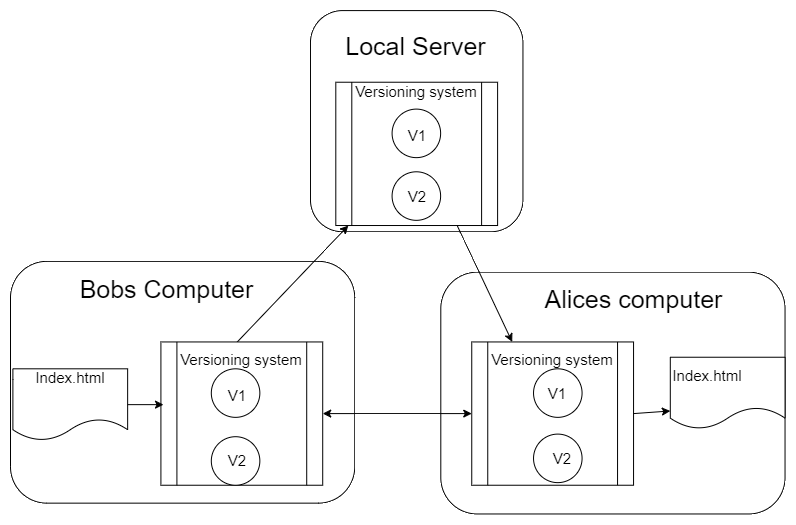
\includegraphics[scale=0.5]{DVCS.png}
\end{figure}

\end{itemize}

\subsection{RCS}

RCS is een klassiek voorbeeld van een lokale versiebeheer systeem. Het wordt geschreven en geformaliseerd door \textcite{Tichy85rcs} in een artikel gepubliceerd aan de universiteit van Purdue in de verenigde staten. GNU -een besturingssysteem dat zeer actief is op het gebied van vrije en democratische software- pikte het project op en voerde het in als een vervanging voor het toenmalige CSSC \autocite{GNUCSSC}. CSSC was een gratis verkrijgbare variant van het SCCS (Source code control system) dat eigendom was van Bell Labs. SCCS is een versiebeheer systeem geschreven door \textcite{Rochkind1975} voor Unix systemen. CSSC en SCCS waren echter niet de enige systemen voor RCS. Zo was er ook nog CA-Panvalet een gepatenteerde oplossing voor Mainframe computers en nog enkele andere.Toch is het interessant om stil te staan bij RCS ten opzichte van eerdere systemen. Veel van de concepten die het systeem omvatte zijn nog steeds terug te vinden in moderne versiebeheer systemen (zoals GIT). RCS kadert eveneens binnen de algemene tendens van deze bachelorproef zo is het volledig open source en kreeg nog een laatste update in 2015.\\

Een eerste concept waar de software gebruik van maakt is het concept van een boomstructuur.
